\documentclass{beamer}

\usepackage{txfonts}
\usepackage{hyperref}
\usepackage{fancybox}
\usepackage{xfrac}
\usepackage{cancel}

\newcommand{\heart}{\ensuremath\heartsuit}

\usepackage{mathtools,amssymb}
\newcommand{\myarrow}{\scalebox{2}[2]{$\mathclap{\curvearrowleft}\mkern2.2mu
                                                 \mathclap{\curvearrowright}$}}



\hypersetup{colorlinks=false,linkbordercolor=red,linkcolor=green,pdfborderstyle={/S/U/W 1}}

\addtobeamertemplate{navigation symbols}{}{ \hspace{1em}    \usebeamerfont{footline}%
    \insertframenumber / \inserttotalframenumber}

\geometry{papersize={15cm,14cm}}
\usepackage{lipsum}

\makeatletter
\newenvironment<>{contdproof}[1][\proofname]{%
    \par
    \def\insertproofname{#1\@addpunct{.}}%
    \usebeamertemplate{proof begin}#2}
  {\usebeamertemplate{proof end}}
\makeatother


\setbeamertemplate{theorems}[numbered]

\newtheorem*{nonumdefinition}{Definition}
\newtheorem*{nonumproblem}{Problem}
\newtheorem*{nonumtheorem}{Theorem}
\newtheorem*{nonumremark}{Remark}
\newtheorem*{nonumsolution}{Solution}
\newtheorem*{nonumexample}{Example}
\newtheorem*{nonumproposition}{Proposition}
\newtheorem{proposition}[theorem]{Proposition}


\usepackage{tikz}
\newcommand*\mycirc[1]{%
  \tikz[baseline=(C.base)]\node[draw,circle,inner sep=.7pt](C) {#1};\:
}

\newcommand\myheading[1]{%
  \par\bigskip
  {\color{blue}{\large #1}}\par\smallskip}

%\usetheme{Warsaw}
%\usetheme{Berkeley} %sample 1
\usetheme{Berlin} % sample 2
%\usetheme{AnnArbor} % sample 3

\let\otp\titlepage
\renewcommand{\titlepage}{\otp\addtocounter{framenumber}{-1}}

\title{Lecture 5 : Independence \S2.5}
\author{}
\date{}

\begin{document}
\begin{frame}[plain]
\titlepage
\end{frame}

\begin{frame}
\begin{nonumdefinition}
Two events $A$ and $B$ are independent if
\begin{equation*}
P(A|B)=P(A)\qquad (\sharp)
\end{equation*}
otherwise they are said to be dependent.
\end{nonumdefinition}
The equation $P(A|B)=P(A)$ says that the knowledge that $B$ has occurred does not effect the probability $A$ will occur.

{\huge $Z$} Remember $P(A|B)$ is defined only if $P(B)\neq 0$
\end{frame}

\begin{frame}
$(\sharp)$ appears to be assymetric but we have

(assuming $P(A)\neq 0$ so $P(B|A)$ is defined and $P(B)\neq 0$ so $P(A|B)$ is defined)

\begin{nonumproposition}
$P(A|B)=P(A)\Leftrightarrow P(B|A)=P(B)$
\end{nonumproposition}

\begin{proof}
\begin{align*}
& P(A\cap B)=P(A)P(B|A)\\[2pt]
& P(B\cap A)=P(B)P(A|B)
\end{align*}
But $A\cap B=B\cap A$ (this is the point)

So
$$
P(A)P(B|A)=P(B)P(A|B)
$$
So
$$
\dfrac{P(B|A)}{P(B)}=\dfrac{P(A|B)}{P(A)}
$$
Then
$$
\text{LHS~}=1 \Leftrightarrow \text{RHS~} =1
$$
\end{proof}
\end{frame}

\begin{frame}
\myheading{The Standard Mistake}

The English language can trip us up here.

Suppose $A$ and $B$ are {\it mutually exclusive} events $(A\cap B=\emptyset)$ with $P(A)\neq 0$ and $P(B)\neq 0$

\smallskip
\centerline{
\includegraphics{figure/fig1.eps}}
\smallskip

Are $A$ and $B$ independent?

\smallskip
\centerline{\Large NO}
\smallskip
$$
P(A|B)=\dfrac{P(A\cap B)}{P(B)}=\dfrac{P(\emptyset)}{P(B)}=\dfrac{0}{P(B)}=0
$$
So\quad $P(A|B)\neq P(A)$.

In this case if you know $B$ has occurred {\it then $A$ cannot occur} at all.

This is the {\it opposite} of independence.
\end{frame}

\begin{frame}
\myheading{Two Contrasting Example}

\myheading{1. Our favorite example}
\begin{align*}
& A=\heart \text{~ on~ } 1^{\text{st}}\\[2pt]
& B=\heart \text{~ on~ } 2^{\text{nd}}\\[2pt]
& P(\heart\text{~ on~ } 2^{\text{nd}} \ | \ \heart \text{~ on~ } 1^{\text{st}})=\dfrac{12}{51}\text{*}
\end{align*}
$P$($\heart\text{~ on~ } 2^{\text{nd}}$ with no other information) = $\sfrac{13}{52}$

So\quad $P(B|A)\neq P(B)$\quad So $A$ and $B$ are {\it not} independent.
\end{frame}

\begin{frame}
\myheading{2. Our very first example}

Flip a fair coin twice
\begin{align*}
& A=H\text{~ on~ } 1^{\text{st}}\\[2pt]
& B=H\text{~ on~ } 2^{\text{nd}}\\[2pt]
& P(H\text{~ on~ } 2^{\text{nd}} \ | \ H\text{~ on~ } 1^{\text{st}})=\dfrac{1}{2}\tag{**}\\[2pt]
& P(H\text{~ on~ } 2^{\text{nd}})=\dfrac{1}{2}
\end{align*}
So\quad $P(B|A)=P(A)$

So $A$ and $B$ {\it are} independent.

Hence
\begin{align*}
P(A\cap B) &= P(A)P(B)\\[2pt]
           &= \left(\dfrac{1}{2}\right)\left(\dfrac{1}{2}\right)=\dfrac{1}{4}
\end{align*}
as we saw in Lecture 1.
\end{frame}


\begin{frame}
\myheading{Remark (don't worry about this)}

Actually in some sense we decided in advance that $A$ and $B$ were independent.

{\it When I give you problems}

{\it you will told whether or}

{\it not $A$ and $B$ are independent.}

When we do ``real-life'' problems we here to decide on a model. In this case in example 1. It is clear that we require a model so that $A$ and $B$ are not independent and in example 2 in which they {\it are}. So we already know the answer to the independence question before doing any mathematics. Again there is something beyond the mathematics.
\end{frame}

\begin{frame}
\myheading{Independence of more than two elements}

\begin{nonumdefinition}
The events $A_{1},A_{2},\ldots,A_{n}$ are independent if for every $k$ and for every collection of $k$ distinct indices $i_{1},i_{2},\ldots,i_{k}$ drawn from $1,2,\ldots,n$ we have 
$$
(b)\quad (A_{i_{1}}\cap A_{i_{2}}\cap\cdots\cap A_{i_{k}})=P(A_{i_{1}})\ldots P(A_{1_{k}})
$$
{\huge Z} So in particular $(k=n)$ we have 
$$
(\sharp)\quad P(A_{1}\cap A_{2}\cap\cdots\cap A_{n})=P(A_{1})P(A_{2})\ldots P(A_{n})
$$
however there are examples where $(\sharp)$ holds but $(b)$ fails for some $k<n$ so the events are not independent.
\end{nonumdefinition}
\end{frame}

\begin{frame}
\myheading{Example $n=3$}

\myheading{Special case of the definition}

Three events $A$, $B$, $C$ are independent if
$$
(\sharp)\quad P(A\cap B\cap C)=P(A)P(B)P(C)
$$
{\it and}
\begin{itemize}
\item[$(b_{1})$] $P(A\cap B)=P(A)P(B)$

\item[$(b_{2})$] $P(A\cap C)=P(A)P(C)$

\item[$(b_{3})$] $P(B\cap C)=P(B)P(C)$
\end{itemize}

{\huge Z} To specialize what I said before there are example where $(\sharp)$ holds but one of the $(b)$'s foils so $(\sharp)$ {\it does not} imply independence.
\end{frame}

\begin{frame}
Now we can easily do the problem from Lecture 1.

$P$(Exactly one head in 100 flips)

Technically we write
$$
A_{i}=H\text{~ on~ } i\text{-th \ flip}
$$
So we want
$$
P(A_{1}\cap A_{2}\cap\ldots\cap A_{100})
$$
by independence
\begin{align*}
&=\underbrace{P(A_{1})P(A_{2})\ldots P(A_{100})}_{100}\\
&= \underbrace{\left(\dfrac{1}{2}\right)\left(\dfrac{1}{2}\right)\ldots \left(\dfrac{1}{2}\right)}_{100}
\end{align*}
It is move efficient to.
\end{frame}

\begin{frame}
\myheading{One of my favorite types of problems (they of to turn up on my tests)}

(see Example 2.35. pg. 79 and problems 80 and 87. pg. 81)

\myheading{System/Component Problems}

\smallskip
\centerline{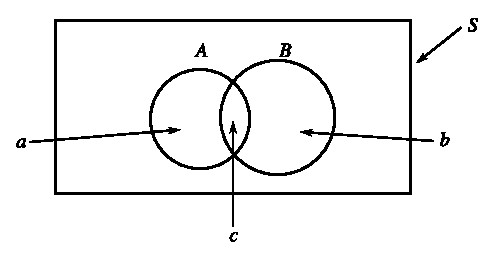
\includegraphics{figure/fig2.eps}}
\smallskip

Consider the following system $S$. Suppose each of the three components has probability $p$ of working. Suppose all components function independently. What is the probability the system will work i.e. an input signal on the left will come out on the right.
\end{frame}

\begin{frame}
\begin{nonumsolution}
It is important that you follow the format below - {\it don't skip steps}. Skipping steps is fatal in mathematics (as in almost everything).
\end{nonumsolution}

\myheading{1. Define events}

$S$ = System works.

$A_{i}$ = $i$-th component works $i=1,2,3$.

\myheading{2. (The hard part)}

{\it Express the set $S$ in terms of the sets $A_{1}$, $A_{2}$, $A_{3}$ using the geometry of the system.}
$$
S=A_{1}\cup (A_{2}\cap A_{3})
$$
???? gets $\Leftrightarrow$ $A_{1}$ works {\it or} (both $A_{2}$ {\it and} $A_{3}$ work) through.
\end{frame}

\begin{frame}
\myheading{3. Use how $P$ interacts with $\cup$ and $\cap$ independence.}
$$
P(S)=P(A_{1}\cup (A_{2}\cap A_{3}))
$$ 
$\cup$ rule
$$
=P(A_{1})+P(A_{1}\cap A_{3})-P(A_{1}\cap (A_{2}\cap A_{3})
$$
independence
\begin{align*}
&=P(A_{1})+P(A_{1})P(A_{3})-P(A_{1})P(A_{2})P(A_{3})\\
&= P+P^{2}-P^{3}
\end{align*}
In a horder problem it is use to group some of the components together in a ``block'' - For example in this problem we could have grouped $A_{2}$ and $A_{3}$ into $C$ so then
$$
S=A_{1}\cup C\qquad\text{etc.}
$$
you should do a lot of these.
\end{frame}

\begin{frame}
When you form the blocks, the blocks will be independent as long as {\it on two blocks have a common component}. So in the example choose $A_{1}$ and $C$ are still independent. 
\end{frame}

\end{document}


